% !TeX root = ../FinalRepordCS.tex

\chapter{Implementation and Preliminary Performance Analysis}

\section{Implementation}
In this section, the main focus is on implementing the functions of LoRa nodes Alice and Bob through the Arduino programmable MCU board and IDE mentioned earlier, in conjunction with the LoRa frequency modulation chip and the algorithms mentioned above.

\begin{figure}
    \centering
    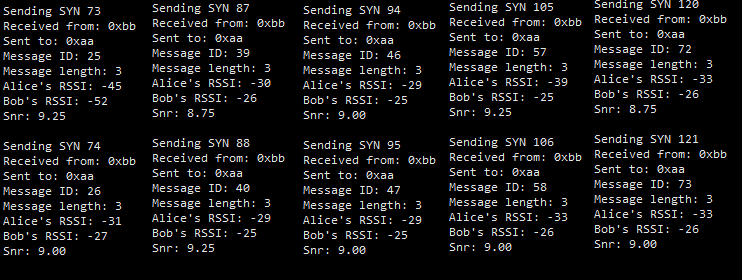
\includegraphics[width=0.9\linewidth]{fig5-1.png}
    \caption{Sampling in LoRa Node}
    \label{fig:5-1}
  \end{figure}

\section{Deep-in-Building and Outdoor Test}
In this section, I conducted a test to generate LoRa physical layer keys in a practical application scenario. The test provided positive results, demonstrating the practical application of LoRa in real-world scenarios. Moreover, the findings are of significant reference value for the future utilization of the LoRa protocol in environmental monitoring.

\subsection{RSSI Pairs Generation}

\subsection{Key Generation}

\subsection{Data Encrypt and Decrypt}

\section{Performance Analysis}
In this section, performance tests on password generation were implemented based on references, exploring the impact of different parameters. Additionally, the results were visualized for better comprehension of the test data.
